\chapter{Documento de Arquitectura de Software}\label{apendice.C}
\section{Introducción}
Este documento brinda una vista general de alto nivel sobre cómo será el desarrollo del sistema JigsawCoding. Se resumirá las tecnologías con las cuales se implementará el sistema así como también se proporcionará una descripción de alto nivel de la arquitectura del sistema.
\subsection{Propósito}
El presente documento de arquitectura de software tiene como finalidad describir el sistema web Jigsaw Coding desde diferentes vistas arquitectónicas, las cuales serán de gran utilidad para el desarrollo de dicho sistema.
\subsection{Alcance} Este documento arquitectónico aplica para describir las características arquitectónicas del sistema web JigsawCoding, las tecnologías que serán usadas en su desarrollo y las principales funcionalidades del sistema.
\subsection{Definiciones, acrónimos y abreviaturas}
En esta sección se provee las definiciones, acrónimos y abreviaturas de términos utilizados en el presente documento a fin de brindar al lector una mejor comprensión del contenido. 
\clearpage
\begin{longtable}{|c|L{8cm}|}
    \hline
  UML & Unified Modeling Language: Lenguaje Unificado de Modelamiento \\ \hline
  CRUD & Create - Read - Update - Delete \\ \hline
  JSON & JavaScript Object Notation: Es un formato ligero para el intercambio de datos \\ \hline
  XML & eXtensible Markup Language: Es un lenguaje de marcas utilizado para almacenar datos en forma legible. \\ \hline
  \emph{sbt} & Herramienta de construcción interactiva \url{http://www.scala-sbt.org} \\ \hline
\end{longtable}
\subsection{Metas arquitectónicas y restricciones}
\subsubsection{Persistencia}
La persistencia se logrará utilizando una base de datos relacional y el mapeo de entidades a tablas estará a cargo del ORM Ebean que por defecto viene incluído en el framework Play.

\subsubsection{Seguridad}
La seguridad del sistema está basada en perfiles. La aplicación contendrá los siguientes puntos:

\begin{itemize}
	\item Autenticación: Cada usuario deberá identificarse con su email y password para poder acceder al sistema.
	\item Autorización: El sistema cuenta con dos perfiles(Docente y Alumno) y dependiendo de ello, el usuario podrá ingresar a diferentes partes del sistema.
\end{itemize}

\section{Representación arquitectónica}
El sistema web JigsawCoding, será implementado usando una arquitectura Modelo - Vista - Controlador, la misma que está definida en el framework Play de Java.
\subsection{PlayFramework 2.2.4}
Play es framework open source de Java y Scala que integra componentes y APIs necesarios para el desarrollo moderno de aplicaciones web. Play sigue el patrón de arquitectura Modelo - Vista - Controlador y uno de sus objetivos es optimizar la productividad del desarrollador a través del uso de configuraciones estandarizadas, recompilación automática del código fuente y la visualización de errores directamente en el navegador.\\

A pesar que las aplicaciones de Play están diseñadas para correr en servidores web basados en Jboos Netty, también pueden ser deployadas como archivos WAR para ser distribuidos en la mayoría de servidores de aplicaciones Java EE como Apache Tomcat o GlassFish.

\subsubsection{Componentes y Características de Play}
\begin{itemize}
  \item JBoss Netty para el servidor web.
  \item Ebean como ORM para Java.
  \item Scala para el motor de plantillas.
  \item Recompilación de código automática.
  \item \emph{sbt} para la administración de dependencias.
  \item CRUD: un módulo para simplificar la edición de objetos.
  \item Secure: un módulo para establecer simples autenticaciones de usuarios.
  \item Parsers de JSON y XML.
  \item Una capa de persistencia basada en JPA
\end{itemize}
\clearpage
\section{Vista Lógica}
\clearpage
\section{Vista de Desarrollo}
La vista de despliegue muestra el sistema desde la perspectiva del programador y se ocupa de la gestión del software a implementar. Esto es, en esta vista se describe cómo estará dividido el sistema JigsaCoding en paquetes y las dependencias que habrá entre ellos.
\begin{figure}[!h]
  \centering
  % Requires \usepackage{graphicx}
  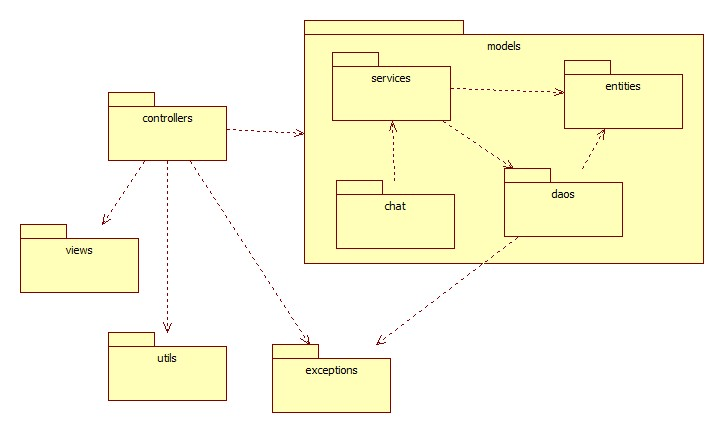
\includegraphics[scale=0.6]{figuras/sad/diagrama_de_paquetes.jpg}\\
  \caption{Diagrama de Paquetes}\label{fig:diagrama_de_paquetes}
\end{figure}
\begin{itemize}
  \item \textbf{controllers}\\Este paquete contiene todas las clases Controladores que sirven para gestionar el ruteo de páginas del sistema.
  \item \textbf{models}\\En este paquete se encuentran las clases de Servicios, Entidades y Acceso a Datos que son requeridas para el sistema.
  \item \textbf{views}\\Este paquete contiene todas las plantillas (\emph{*.scala.html}) que permitirán renderizar las páginas web del sistema.
\end{itemize}
\clearpage
\section{Vista Física}
\begin{figure}[!h]
  \centering
  % Requires \usepackage{graphicx}
  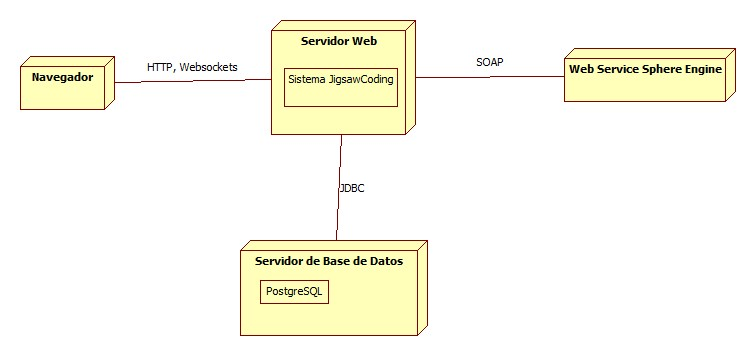
\includegraphics[scale=0.5]{figuras/sad/diagrama_de_despliegue.jpg}\\
  \caption{Diagrama de Despliegue}\label{fig:diagrama_de_despliegue}
\end{figure}
\begin{itemize}
  \item \texttt{Navegador}\\Es la interfaz que permitirá visualizar el contenido de las páginas web del sistema JigsawCoding.
  \item \texttt{Servidor Web}\\Es el responsable de gestionar todas las peticiones HTTP provenientes de los navegadores web y de enviar las respuestas con los datos solicitados por los mismos.
  \item \texttt{Servidor de Base de Datos}\\Es el lugar donde estará almacenada la información del Sistema Web JigsawCoding
  \item \texttt{Web Service Sphere Engine}\\Es un servicio web que servirá para compilar y ejecutar el código fuente desarrollado por los usuarios del sistema.
\end{itemize}
\clearpage

\begin{landscape}
\section{Vista de Escenarios}
La vista de escenarios o vista de casos de uso es la encargada de presentar la percepción que tiene el usuario sobre las distintas funcionalidades del sistema.
\begin{figure}[!h]
  \centering
  % Requires \usepackage{graphicx}
  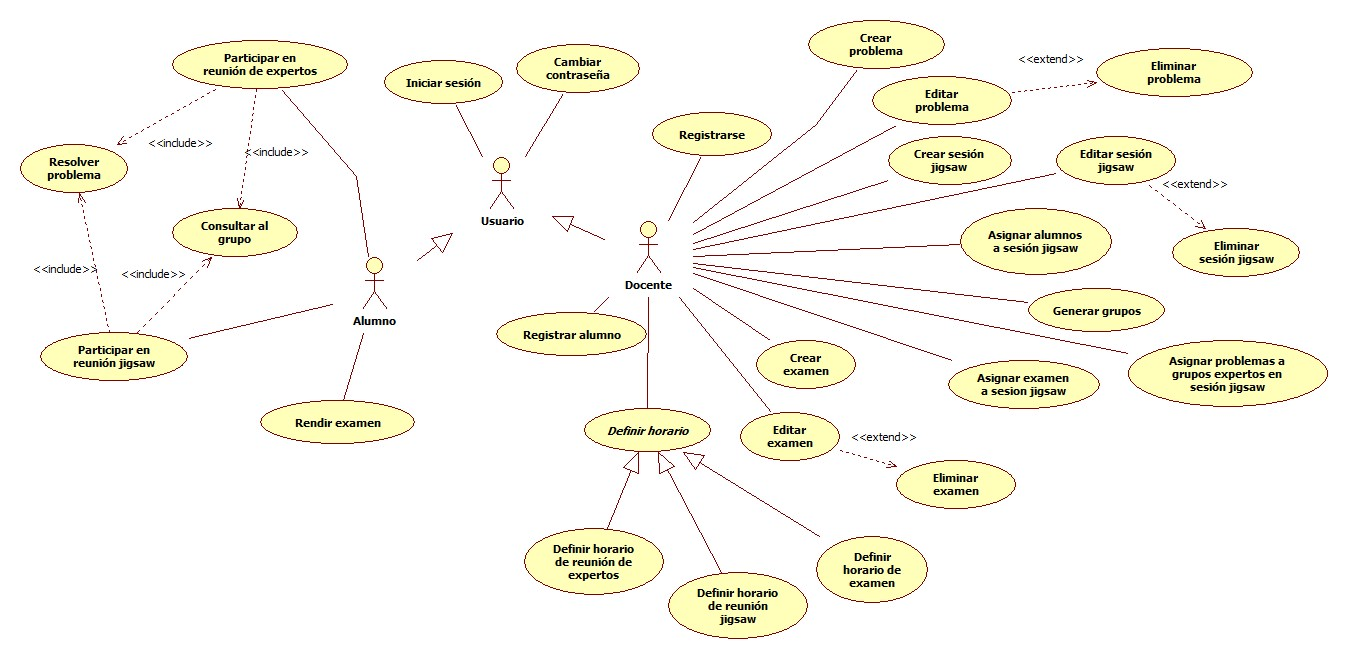
\includegraphics[scale=0.45]{figuras/casosdeuso/casos_de_uso.jpg}\\
  \caption[Casos de uso]{Diagrama de casos de uso para el sistema JigsawCoding}
  \label{fig:casos_de_uso}
\end{figure}
\end{landscape}
\clearpage
\section{Vista de Datos}
\begin{figure}[!h]
  \centering
  % Requires \usepackage{graphicx}
  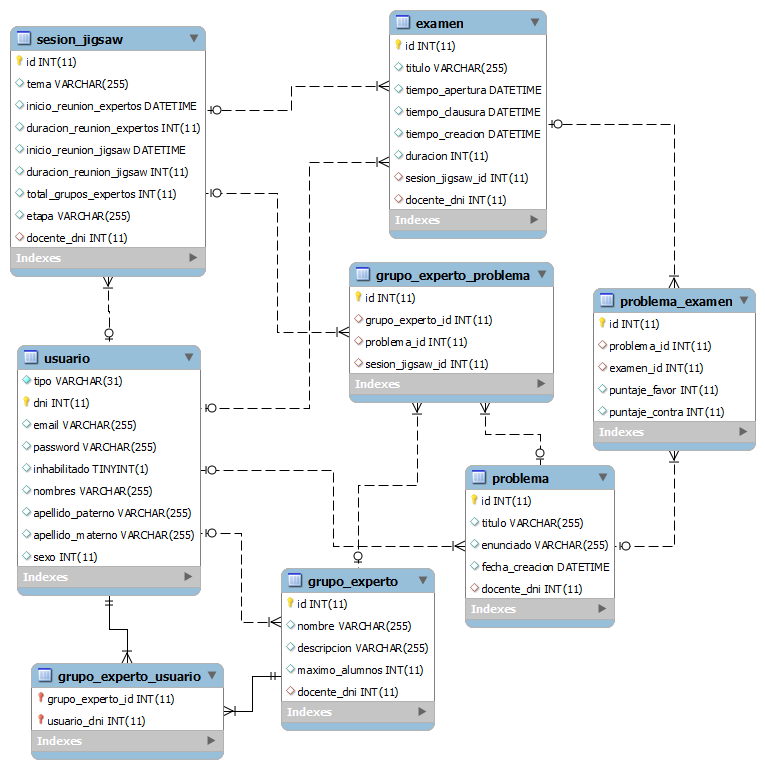
\includegraphics[scale=0.6]{figuras/sad/modelo_de_datos.png}\\
  \caption[Modelo de datos]{Modelo de base de datos del sistema JigsawCoding}\label{fig:modelo_de_datos}
\end{figure}
\subsection{MySQL 5.6}
El desarrollo del sistema JigsawCoding se hará usando como motor de base de datos a MySQL en su versión 5.6. Este, es un sistema de gestion de base de datos libre actualmente soportado por Oracle. 
\subsection{Diccionario de datos}